\section{Economic Framework and Measurement}
\label{sec:setting}

\subsection{Cross-country configurations as information}

Let the 10-year/2-year slope in country $i$ be
\begin{equation}
    q_{i,t}=\mu_i+f_t+u_{i,t},
    \label{eq:slope_information}
\end{equation}
where $\mu_i$ is a country level, $f_t$ is information shared across curves, and $u_{i,t}$ collects country-specific information and measurement error. A lower $f_t$ tends to flatten several curves. The inversion indicator is
\begin{equation}
    I_{i,t}=\1\{q_{i,t}<0\}.
    \label{eq:inversion_threshold}
\end{equation}
One threshold crossing can arise from either component. Several fresh crossings are harder to attribute to one country's $u_{i,t}$. This signal-extraction logic requires restrictions on the cross-country dependence of the country-specific components: regional shocks, coordinated policy, or common measurement errors can also produce synchronization. Equations~\eqref{eq:slope_information}--\eqref{eq:inversion_threshold} therefore motivate empirical comparisons; they do not identify $f_t$ or assign a structural posterior probability to two crossings.

The framework yields a nonlinear prediction. Exactly one inversion need not be a weaker adverse state than two. A single curve can identify a national rate cycle, whereas a cluster can change the composition of likely information. It also yields a spanning prediction: if the cross-country configuration matters, it should add information beyond one country's curve and a continuous average slope. The threshold and path rules are empirical measurements of that configuration, not primitives of the model.

The yield-slope component and the subsequent currency-return innovation are distinct. Write
\begin{equation}
    \Delta s_{i,t+1}=-\lambda_i h_{t+1}+e_{i,t+1},
    \label{eq:factor_decomposition}
\end{equation}
where $h_{t+1}>0$ is an adverse return component shared across currencies, $\lambda_i$ is currency $i$'s exposure, and $e_{i,t+1}$ is idiosyncratic. The synchronized state is informative when $\E[h_{t+1}\mid S_t=1]$ exceeds its inactive-state counterpart. Equation~\eqref{eq:factor_decomposition} then predicts larger depreciations for high-$\lambda_i$ currencies. Predetermined equity beta is the empirical exposure proxy. The paper does not equate $f_t$ with $h_{t+1}$; the first is information in bond-market configurations, and the second organizes the currency payoff.

\subsection{Currency returns and the shared-loss problem}

Consider a U.S. investor holding currency $i$. Let $s_{i,t}$ be the log dollar price of one unit of foreign currency, so $\Delta s_{i,t+1}>0$ is foreign-currency appreciation. Let $d_{i,t}\equiv(i_{i,t}-i_{US,t})/12$ be the one-month interest differential, formed from annualized money-market rates. The excess-return proxy is
\begin{equation}
    rx_{i,t+1}=d_{i,t}+\Delta s_{i,t+1}.
    \label{eq:currency_return}
\end{equation}
The differential is known at $t$; the spot change is realized from $t$ to $t+1$. Under covered interest parity this sum corresponds approximately to a forward return apart from basis and measurement differences \citep{du2018}. It combines a simple annualized interest-rate differential divided by twelve with a log spot change, a first-order monthly approximation. Because the paper uses money-market differentials rather than executable forward quotes, the object is an asset-pricing return proxy, not a transaction-cost-adjusted strategy.

Each month, the carry portfolio buys the three highest-rate currencies and sells the three lowest-rate currencies among the nine non-dollar G10 currencies. If $\mathcal H_t$ and $\mathcal F_t$ denote the high-rate and funding sets, then
\begin{equation}
\begin{aligned}
    rx^{\mathrm{carry}}_{t+1}
      &=\frac{1}{3}\sum_{i\in\mathcal H_t}rx_{i,t+1}
       -\frac{1}{3}\sum_{i\in\mathcal F_t}rx_{i,t+1} \\
      &\equiv C_t+X_{t+1}.
\end{aligned}
\label{eq:carry_return}
\end{equation}
Here $C_t$ is the long-minus-short interest differential and $X_{t+1}$ is the corresponding spot return. The sample-average income leg is 3.9 percent per year and is positive in every month, with a minimum of 0.7 percent. Carry therefore loses only when the spot leg is more negative than the income leg is positive.

Diversification reduces $e_{i,t+1}$ but not the shared component when the long and funding legs have different average exposures. Here ``shared'' describes cross-currency comovement; ``international'' is the economic interpretation. The return equation is an organizing device rather than an estimated factor model.

\subsection{The synchronized-inversion state}

Let $q_{i,t}\equiv y^{10Y}_{i,t}-y^{2Y}_{i,t}$ denote country $i$'s end-of-month yield slope. An inversion can reflect expected easing, term-premium variation, or both \citep{campbellShiller1991,hamiltonKim2002,bauerMertens2018}.

Define $I_{i,t}=\1\{q_{i,t}<0\}$. A crossing observed at $t-1$, $I_{i,t-2}=0$ and $I_{i,t-1}=1$, makes the curve live at $t$. It remains live until $q_{i,t}$ has increased for two consecutive months. A released curve cannot re-enter while still inverted; it must first become nonnegative and then cross below zero again. Let $L_{i,t}$ be the resulting live status. The central state is
\begin{equation}
    N_t=\sum_{i=1}^{9}L_{i,t},
    \qquad
    S_t=\1\{N_t\geq2\}.
    \label{eq:signal}
\end{equation}
Thus $L_{i,t}$ is path dependent, whereas $I_{i,t}$ depends only on the current slope. The state measured at the end of month $t$ conditions the return during month $t+1$.

The live rule has two economic roles. Delayed fresh entry excludes inversions already embedded in prices for many months and prevents the crossing-month return from entering the predictive state. Confirmed release allows the state to remain active as curves re-steepen, which can coincide with delivered easing and delayed currency adjustment. In the sample, a raw two-or-more current-inversion state is active in 165 months, compared with 92 for the live state, yet switches off before March 1995, October 2008, and March 2020---the three largest carry-loss months. This historical fit is informative and also creates specification-search risk. Online Appendix A states the transition rules and boundary cases exactly.

\begin{figure}[p]
    \centering
    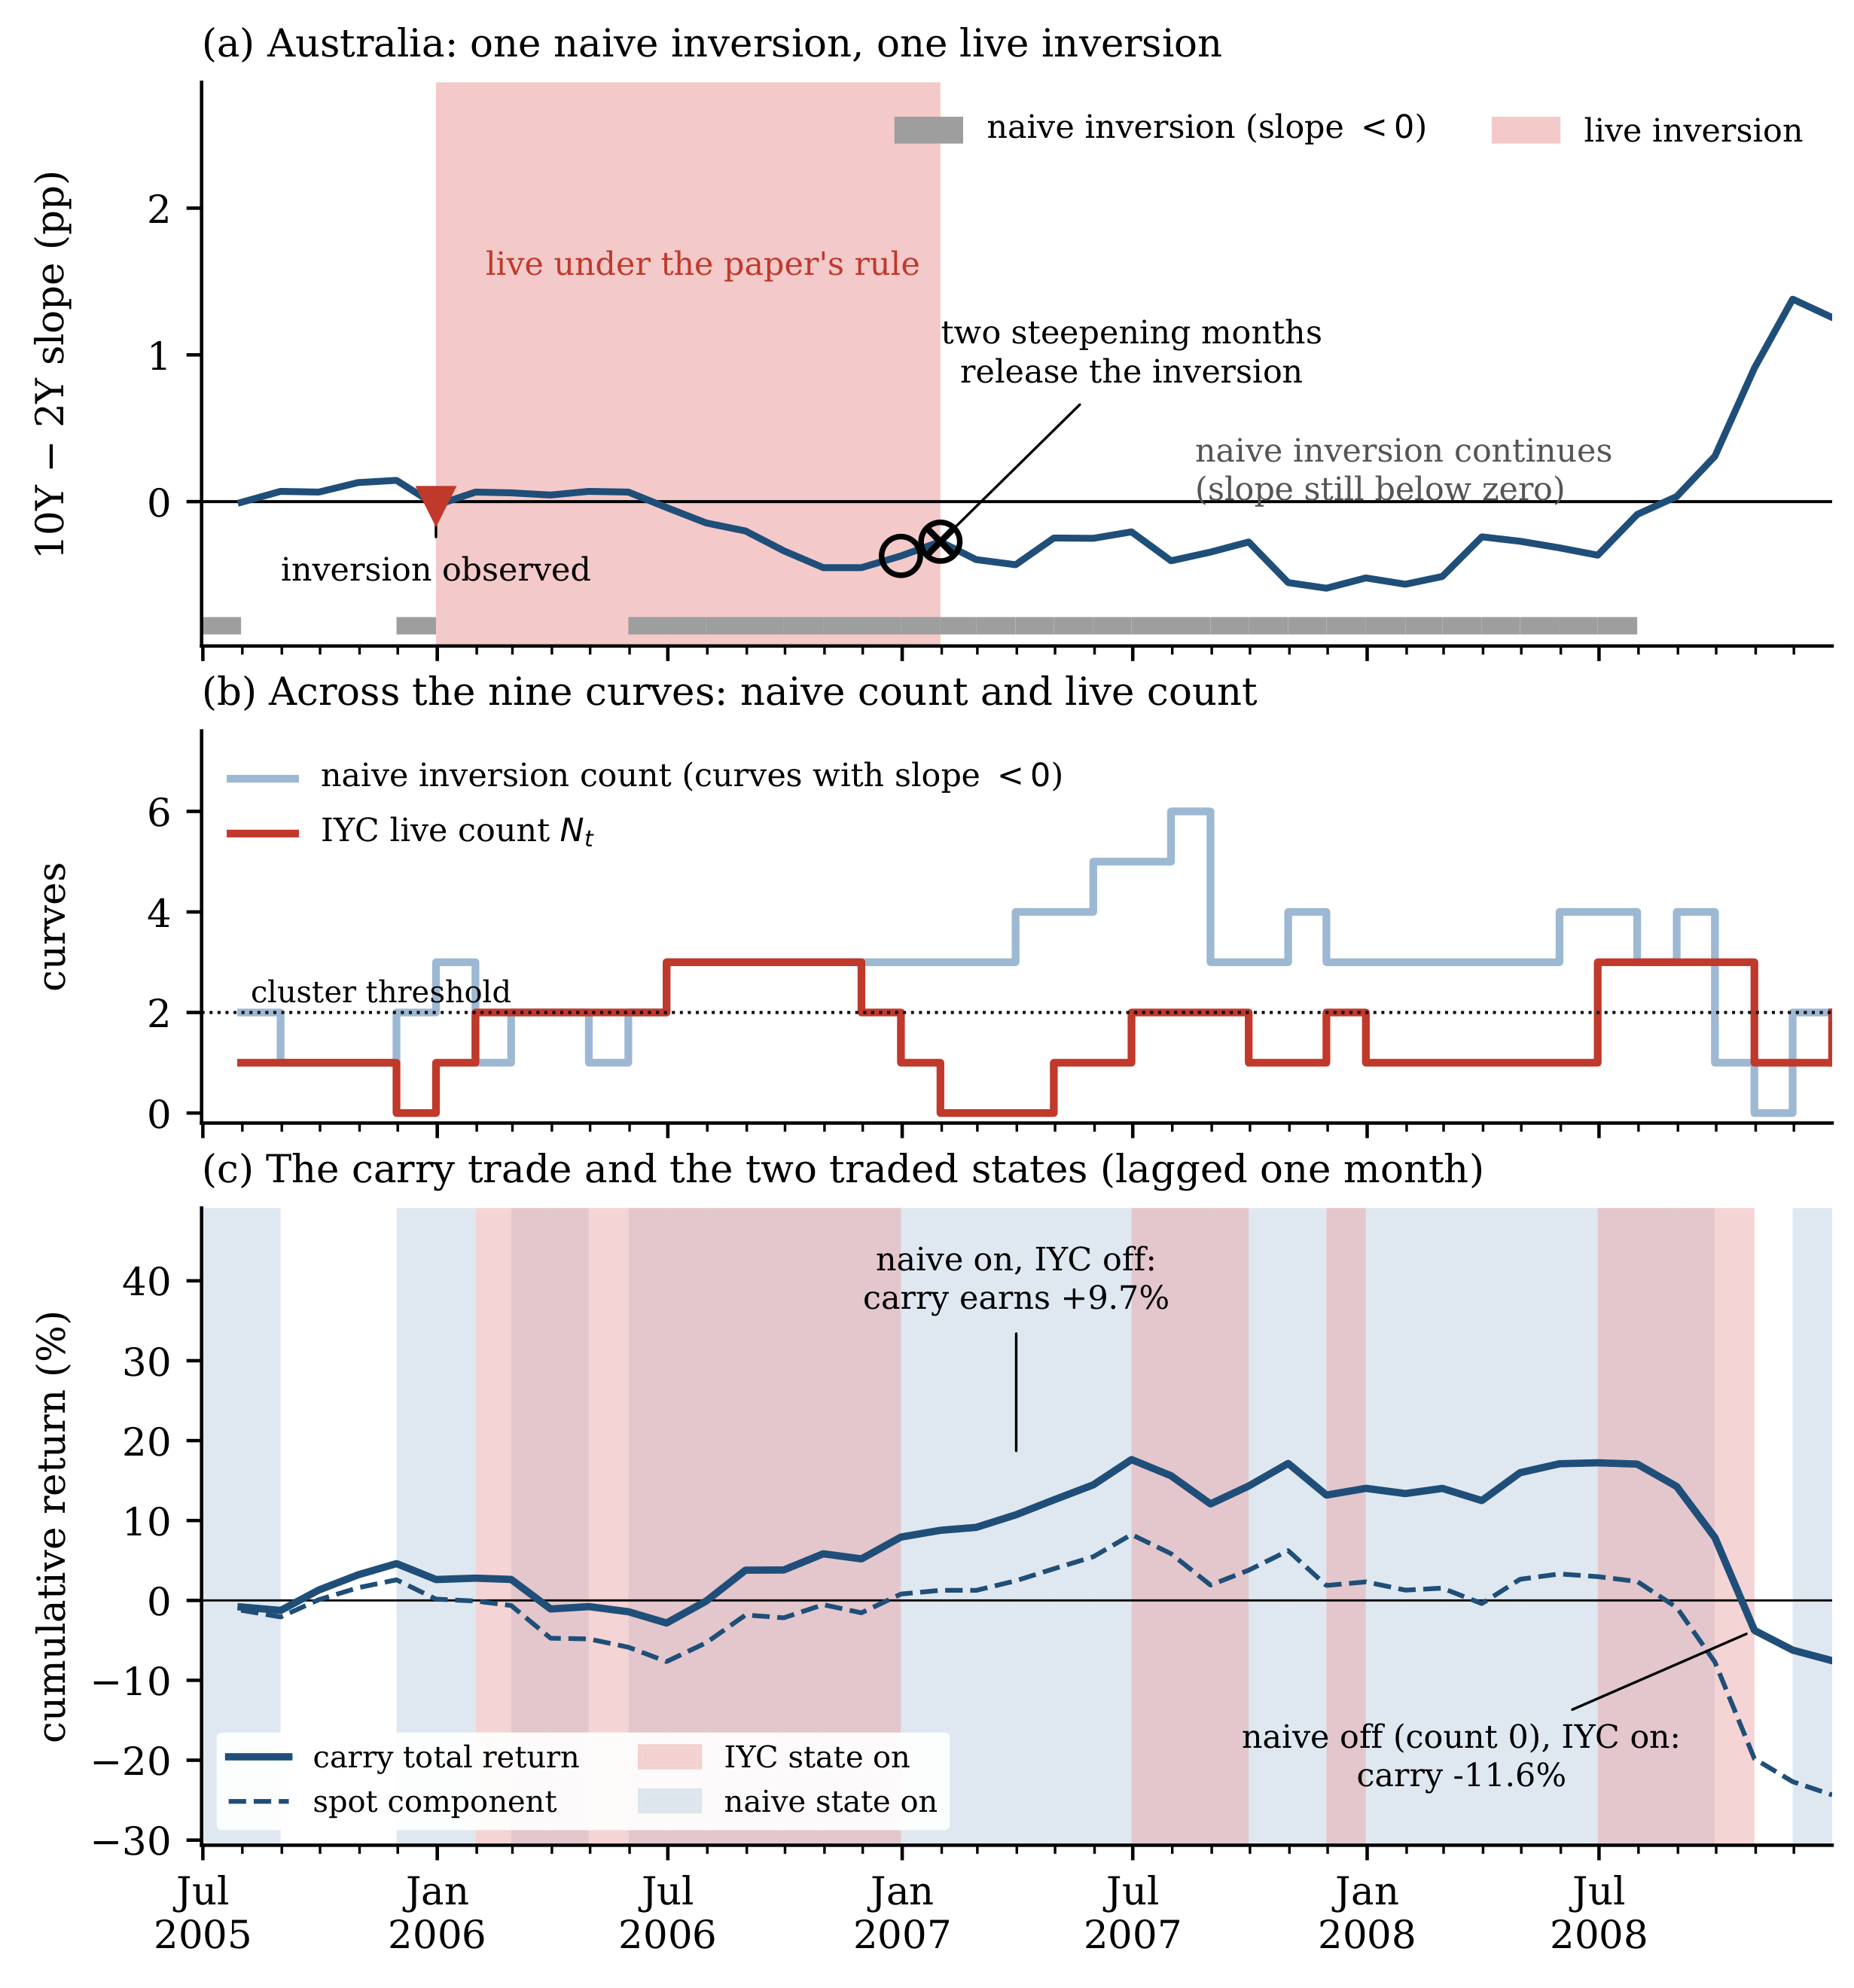
\includegraphics[width=\textwidth]{assets/original/figure_02_main.png}
    \caption{Live-state construction, 2005:07--2008:12. Panel (a) shows the Australian 10Y--2Y slope and its live status, which begins one month after the crossing is observed. Panel (b) compares the current-inversion and live counts. Panel (c) plots cumulative carry returns under the two lagged states. Delayed fresh entry removes the crossing-month return and stale inversions; confirmed release can retain the state after the current-inversion count declines.}
    \label{fig:inherited_latch}
\end{figure}

\subsection{Data, information set, and predetermined exposure}

The monthly sample runs from January 1988 through February 2026. The currency universe comprises the Australian dollar, Canadian dollar, Swiss franc, euro (Deutsche mark before 1999), British pound, Japanese yen, Norwegian krone, New Zealand dollar, and Swedish krona. The dollar is the numeraire and does not enter either the sort or the baseline state count. The U.S. curve is retained as a benchmark.

State incidence varies across monetary regimes. It is active in 33 of 84 months during 1988--94 but only 3 of 120 months during 2010--19, when many policy rates were near their lower bounds. The state is not a continuously available factor; it appears when international rate cycles create enough cross-country slope variation. Online Appendix A reports the full era counts.

The baseline state uses end-of-month 2-year and 10-year government yields. Portfolio weights use one-month money-market rates known at $t$. Return regressions use no information dated after $t$ to predict month $t+1$. This convention prevents mechanical look-ahead but does not eliminate asynchronous market closes, stale quotes, or later data revisions.

The exposure test estimates a currency's equity beta on an expanding window:
\begin{equation}
    rx_{i,\tau}=a_i+\widehat\beta_{i,t}r^M_{\tau}+u_{i,\tau},
    \qquad \tau\leq t-1.
    \label{eq:currency_beta}
\end{equation}
The estimate $\widehat\beta_{i,t}$ is available before the return from $t$ to $t+1$ and requires at least 36 prior monthly observations. The one-month buffer is part of the baseline construction: the estimate paired with $S_t$ uses currency and equity returns only through $t-1$. The beta is an empirical proxy for the latent exposure $\lambda_i$ in equation~\eqref{eq:factor_decomposition}; it need not equal that primitive. S\&P 500 total returns form the market measure.

\begin{table}[H]
\centering
\caption{Notation and timing}
\label{tab:notation}
\small
\begin{tabularx}{\textwidth}{>{\raggedright\arraybackslash}p{2.1cm} >{\raggedright\arraybackslash}X >{\raggedright\arraybackslash}p{3.0cm}}
\toprule
Symbol & Definition & Timing \\
\midrule
$t$; $t+1$ & Information month-end; subsequent holding month & Information $\rightarrow$ return \\
$s_{i,t}$; $\Delta s_{i,t+1}$ & Log dollar price of currency $i$; its one-month change & Spot change realized in $t+1$ \\
$d_{i,t}$ & Monthly foreign-minus-U.S. interest differential & Known at $t$ \\
$rx_{i,t+1}$ & Currency excess-return proxy & Realized in $t+1$ \\
$C_t$; $X_{t+1}$ & Carry income leg; carry spot leg & Known at $t$; realized in $t+1$ \\
$q_{i,t}$ & Country $i$'s 10Y--2Y yield slope & Observed at month-end $t$ \\
$I_{i,t}$; $L_{i,t}$ & Current inversion; path-dependent live inversion & Information at $t$ \\
$N_t$; $S_t$ & Live-curve count; synchronized-inversion state & Predict $t+1$ \\
$f_t$; $h_{t+1}$ & Shared slope information; adverse currency-return component & Information at $t$; payoff in $t+1$ \\
$\lambda_i$; $\widehat\beta_{i,t}$ & Latent return exposure; estimated equity-beta proxy & Beta uses data through $t-1$ \\
$W_t$ & Vector of lagged benchmarks or controls & Known at $t$ \\
\bottomrule
\end{tabularx}
\begin{minipage}{0.94\textwidth}
\footnotesize\emph{Notes:} Equations use the information-time convention $t\rightarrow t+1$. Tables indexed by the return month equivalently report $S_{t-1}$.
\end{minipage}
\end{table}
